\chapter{Estrutura}
\label{cap:Estrutura}

Para conceber a arquitectura do sistema de monitorização de rede de um processo, foi necessário conhecer como os processos comunicam com o exterior.
 Conhecendo a arquitectura de rede do \textit{Linux}, foi necessário perceber de que forma se processa a captura dos dados transmitidos e/ou recebidos pela interface de rede. 

Neste capitulo vai ser apresentado a constituição do sistema de rede do \textit{Linux}, desde o momento em que a aplicação envia os dados, até ao momento em que estes chegam à interface de rede e vice-versa.
Como esta visão é muito abrangente, apenas serão focados os pontos essenciais da arquitectura.
Após esta visão geral do sistema, é apresentado a arquitectura do projecto desenvolvido.


\section{Arquitectura de rede em \textit{Linux}}
\label{subsection:network}
Um processo para poder comunicar remotamente com outro processo em outra máquina remotamente irá utilizar as funcionalidades de rede do seu sistema de operação.
 Para isto um processo tem de efectuar o inicio da comunicação enviando alguns pacotes de inicio de sessão (caso o protocolo de comunicação necessite).
 Um processo em \textit{Linux} é uma instância de um programa que partilha da máquina e que pode comunicar com outros processos.
 Os processos dentro do núcleo são instâncias de uma estrutura \textit{task\_struct} que contém diversos elementos pertencentes ao processo, tais como identificador de processo, ficheiros abertos no sistema de ficheiros, zonas de memória que lhe foram atribuidas, etc.
 
 Um processo para utilizar as funcionalidades de rede necessita criar uma instância de um socket em o indicador devolvido ao processo é um descritor de ficheiros (descritor de socket).
 Isto porque os \textit{sockets} de um processo são mapeados em um sistema de ficheiros virtual neste caso sobre a forma de sockets, forma de comunicação sobre a rede.
 Estes descritores permite ao processo identificar o socket e efectuar as comunicações.
 Estas comunicações, bem como o estabelecimento destes canais de comunicação, são efectuadas através de chamadas ao sistema de operação.

A arquitectura de rede do núcleo do \textit{Linux} poderá ser apresentada de duas formas, \textit{Bottom-Top} ou \textit{Top-Bottom}. 
A escolha recaíu sobre a primeira pois permite observar o aumento da complexidade e abstracção existente nesta arquitectura. 

Falar aqui sobre qq coisa da estrutura de rede ... 
Talvez tb imagem com um pouco da arquitectura ... básica 

Falta falar sobre o netfilter ... sobre tc trafic control

Socket  e o que é um socket ...

Os ``file descriptors'' são a abstração para os ``sockets''. Os sockets são
mapeados em ficheiros e estes em descritores de ficheiros. 

Dentro do núcleo do linux a estrutura que tém a informação sobre um processo
(\textit{task}), é a \textit{struct task\_struct}. Nesta estrutura existe a
informação sobre quais os ficheiros que a aplicação abriu. Como os
\textit{sockets} são mapeados sob a forma de ficheiros, estes também se
encontram nesta estrutura.

Os protocolos \textit{TCP} e \textit{UDP} foram os únicos protocolos que se teve
interesse em utilizar nesta ferramenta.

Estes protocolos estão definidos numa estrutura de apontadores para funções.
Os protocolos \textit{TCP} e \textit{UDP} têm formas diferentes de executar
funcionalidades semelhantes e por isso estão descritos em instâncias diferentes.

As principais chamadas ao sistema para estabelecer, terminar e transferir dados
sobre \textit{sockets} são: \textit{socket}, \textit{connect}, \textit{bind},
\textit{listen}, \textit{accept}, \textit{send}, \textit{recv}, \textit{sendto},
\textit{recvfrom} e \textit{close}. 

Estas chamadas aos sistema são genéricas de forma a poderem ser mapeadas nas
diferentes instâncias dos protocolos de transferência

Quando a chamada ao sistema \textit{socket} é efectuada, é criado uma nova
instância de um socket e inicializados os respectivos campos com a informação
dependente para a familia e tipo. 

%  Descrever um pouco esta parte ...

Como os protocolos \textit{TCP} e \textit{UDP} partilham algumas das
funcionalidades nem todas as f




\subsection{Estrutura de um processo}

Um processo para executar tem de ser carregado para memória e posteriormente ser agendado para execução através do escalonador de processos do núcleo.
 Um processo para o núcleo é uma estrutura com a informação sobre as zonas de memória, descritores de ficheiros abertos, informações sobre os tempos de execução, informações sobre a hierarquia de processos pertencentes a este, etc. Nos descritores de ficheiros abertos são também incluidos os descritores de \textit{sockets} abertos para comunicação. 

\subsection{Sistema de ficheiros}

Um processo para poder comunicar com a interface de rede tem de abrir um canal entre o processo e o núcleo de operação que por sua vez comunica com a interface de rede.
 Este canal nos sistemas de operação \textit{Linux} é efectuado através da chamada ao sistema \textit{socket}.
 Esta função regista a abertura de um canal de comunicação entre o processo e o sistema de rede, sendo o descritor do \textit{socket} um identificador do sistema de ficheiros, que fica registado no descritor do processo dentro do núcleo.
 Esta é apenas a primeira das abstrações que o núcleo efectua sobre a arquitectura do sistema de rede.
  
algures falar sobre o accept e o bind e o socket devido à estrutura interna que aguarda o indicador da porta igual ... tenho de verificar isto correctamente




\subsection{Interfaces de rede}

O núcleo do \textit{linux} mantém a informação sobre quais as interfaces de
rede que foram inicializadas pelos seus controladores, mesmo que não estando
activas estas constantam de uma lista duplamente ligada de
\textit{net\_devices}. Em cada posição da lista está toda a informação
referente a uma interface de rede e suas configurações, nomeadamente a
informação sobre o seu endereço ip ou o seu mac address no caso de interfaces
\textit{ethernet} ou mapeadas sobre \textit{ethernet} (como o caso das
interfaces ponto-a-ponto).
 
\subsection{Estrutura de um sk\_buff}

\subsection{NetFilter}

O sistema de operação \textit{Linux} tem um sistema de \textit{firewall} que permite controlar os acessos dos processos aos sistemas de comunicação de rede.
 Este sistema é o \textit{NetFilter}, está presente no núcleo do sistema operação permitindo controlar o fluxo de dados dos processos para as interfaces de rede, bem como no sentido oposto. O \textit{NetFilter} está presente na \textit{stack TCP/IP} em 5 pontos apenas e desta forma consegue de uma forma simples controlar o fluxo dos dados. O \textit{NetFilter} pode ser controlado pelo \textit{iptables}, uma ferramenta em nível utilizador que através de regras define o acesso dos dados das comunicações rede.

\subsection{Traffic Control}
Apesar de ter estrutra para controlo dos dados que chegam da interface de rede o principal propósito é controlo do dados que saem da interface.



\subsection{AF\_PACKET}

A forma para comunicar enviar e receber dados directamente da interface de rede
é através da familia de protocolos \textit{AF\_PACKET}. 

Esta é a forma de implementar protocolos de rede sem recorrer à \textit{stack}
de protocolos IP em nível utilizador. Para além desta funcionalidade esta é a
forma de capturar os pacotes que circulam na interface de rede, permitindo
assim efectuar uma análise do tráfego.

Esta camada situa-se junto aos controladores de rede permitindo assim capturar
dados que podem não chegar às aplicações devido à utilização de regras na
\textit{firewall} (netfilter) do \textit{linux}.

A utilização de ``lazy cloning'' permite que apenas os pacotes que sejam para
capturar sejam efectivamente copiados. Por isso primeiro são avaliados para o
processo de captura, caso sejam para captura a função \textit{blah blah}
efectua a cópia da estrutura sk\_buffer e serão então adicionados ao
\textit{ring buffer}. Se no \textit{ring buffer} não existir espaço para o
número de bytes que devem ser capturados, é então descartado a cópia
(libertado o espaço) e incrementado o valor de pacotes descartados pelo núcleo
de sistema.

\subsection{Recepção de dados}

A chegada de um pacote de dados à interface de rede desencadeia uma acção de interrupção da actividade do processador, permitindo quer este seja transferido para o sistema o mais cedo possível. Esta interrupção é efectuada através de um \textit{irq} pré-definido entre o controlador e a interface de rede. As interrupções são atendidas no processador desligando a atenção a todas as outras interrupções provenientes de outros dispositivos. %esta frase está ruim ...
O processador deve estar o menor intervalo de tempo possível com as interrupções desligadas, antes de retornar da interrupção o sistema agenda a execução de uma função que irá terminar a recepção do pacote para a camada correcta da \textit{stack TCP/IP}.%ainda falta falar sobre DMA, interrupt mode too exclusive deve ser breve, encaminhar pelo processamento da stack tcp/ip 

No processo de recepção da \textit{frame} é verificado se existem \textit{sniffers} registados, caso existam é passada uma referência sobre a frame, de forma a efectuar apenas a cópia da frame quando necessária. Esta situação é devida à possível existência de um filtro sobre a \textit{frame}, em que se não for necessário capturá-la, a cópia dos dados seja desnecessária, permitindo efectuar trabalho útil.

%Faltar falar que a frame segue para a stack tcp ip de forma normal ...

%Falta falar sobre o netfilter ... firewall do linux que existem 5 pontos de "entrada" onde existe algumas verificações .... 

% Faltar indicar que o processo está bloqueado à espera de input que lhe é copiado entre o nucleo e o processo em nivel utilizador por meio de o kiovec (talvez kernel io vector ...) 


A variável global \textit{ptype\_base} do núcleo é uma tabela de dispersão aberta, que contém os tipos de controladores de protocolos de rede. Os diferentes protocolos endereçam uma função que recebe o pacote e sabe o que fazer com ele, passando pela \textit{firewall netfilter} terminando na cópia dos dados dos \textit{buffers} do núcleo para os do processo, que ficou bloqueado numa lista de espera através da chamada ao sistema de operação \textit{recv}, \textit{recvfrom} ou \textit{recvmsg}.

\subsection{Transmissão de dados}

Uma aplicação em nível utilizador transfere dados sobre a rede através de chamadas ao sistema de operação, sendo que estas podem ser \textit{send}, \textit{sendto}, \textit{sendmsg}.
 Neste ponto de entrada os dados tem de ser copiados e efectuadas diversas verificações sobre estes, após estas verificações são utilizadas estruturas e funções através da \textit{stack TCP/IP} e fluir pela \textit{firewall netfilter}.
 Os dados gerados pelas diversas camadas da \textit{stack} são agregados numa estrutura \textit{sk\_buffer} para ser adicionados a uma fila para ser enviados pela ferramenta \textit{traffic control}.
 Quando esta ferramenta irá enviar os dados para o controlador é passada a referência sobre este pacote para os \textit{sniffers} registados, sendo apenas efectuada uma cópia dos dados caso o pacote seja recolhido para maior análise. Os dados passados ao controlador da interface de rede são então transferidos para a interface de rede, e daí para o seu destino.

Quando a aplicação está a executar e efectua uma chamada ao sistema de operação, o sistema muda de modo e executa dentro do núcleo "em nome da aplicação".
 Durante parte da execução da chamada ao sistema de operação é possível referenciar qual o processo que efectuou a chamada, pois caso a chamada seja sincrona, é agendada um processamento sobre os dados e a aplicação fica bloqueada à espera de ser re-escalonada através da função \textit{schedule}.
 O sistema de ficheiros mantém a referência sobre quais os ficheiros/sockets abertos para cada processo e é possível obter qual o processo a que cada descritor de ficheiros pertence. % back pointers ... nos sockets ... binded de uma porta a um processo ... pode nao ser a chamada bind ... 

\section{Desenho e arquitectura}
\label{sec:architecture}

O sistema proposto foi desenvolvido procurando cumprir os seguintes requisitos:
\begin{itemize}
\item permitir seleccionar as comunicações envolvendo apenas um processo (ou um conjunto de processos);
\item manter a compatibilidade com o sistema já existente, estendendo a sua funcionalidade;
\item procurar minimizar eventuais percas de desempenho;
\item a implementação deve envolver poucas alterações ao código do sistema, para facilitar a sua manutenção e evolução com as novas versões do sistema Linux.
\end{itemize}

Para tal, o sistema criado está dividido em 4 componentes principais (ver figura \ref{arquitectura}). A função de filtragem, invocada por um \textit{hook} que estende o LSF, permite que apenas o tráfego do processo alvo seja analisado pelo restante sistema de fitragem do LSF. Uma componente de instrumentação das chamadas ao sistema (ou outras funções contidas no sistema de rede) que actualiza o repositório de dados onde é mantido o estado das interacções via rede do(s) processo(s) alvo. Existe ainda um sistema para controlo/configuração e para obter informação do estado da monitorização.

\begin{figure}[htbp]
\begin{center}
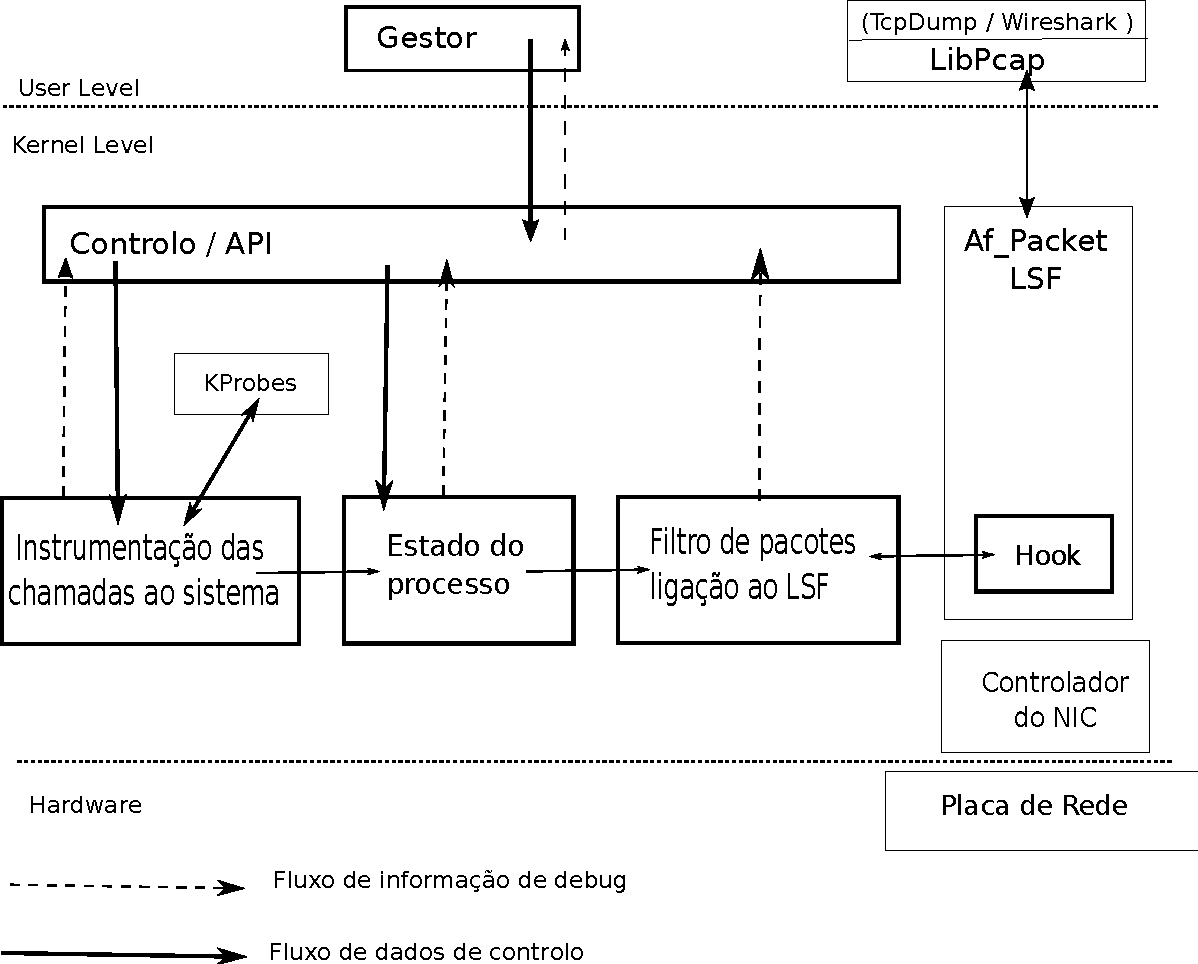
\includegraphics[scale=0.5]{interface.pdf} 
\caption{Arquitectura da solução}
\label{arquitectura}
\end{center}
\end{figure}


Este sistema permite que sejam capturados os pacotes de rede de um processo, sem que exista um conhecimento prévio sobre o(s) protocolo(s) ou portas utilizadas. A utilização de um sistema de instrumentação do núcleo foi necessária apenas para monitorizar as chamadas envolvendo \emph{sockets} e identificar o processo responsável, permitindo desta forma obter e manter permanentemente actualizada a informação sobre o estado respeitante ao processo alvo. De forma a minimizar a redução de desempenho, todo o sistema foi desenvolvido dentro do núcleo do \textit{Linux}, sem alterações nas interfaces já existentes.  Assim, ferramentas de façam uso da biblioteca \textit{LibPcap}, como o programa \textit{tcpdump} ou suas variantes, podem beneficiar desta extensão sem qualquer alteração e sem impacto relevante no seu desempenho.

---------------------------------------------------------------------------------------------------------

A arquitectura foi pensada para ser executada de forma ortogonal ao sistema
utilizado. Desta forma não existe a necessidade de recompilar programas
antigos. Para além desta situação novas aplicações podem utilizar esta
ferramenta de forma transparente.

Esta ferramenta foi desenvolvida para os processadores x86 e x86\_64 pois nestas
arquitecturas existe suporte para o sistema de monitorização KProbes \ref{},
sendo esta a unica dependência especifica que a ferramenta irá ter.

As diferentes partes da ferramenta foram desenvolvidas de forma a poderem ser
modificadas em separado permitindo um melhor aproveitamento da modularização.
Este módulo foi desenvolvido em 4 subpartes. 

---------------------------------------------------------------------------------------------------------


\subsection*{Instrumentação das chamadas ao sistema de rede}
\label{sub:mon_syscalls}

Um ponto importante deste sistema, constituiu na garantia que todas as interacções desencadeadas por um processo com o exterior fossem detectadas. Para tal, foi necessário recorrer à monitorização das chamadas ao sistema de rede ao nível do Kernel, permitindo, assim, minimizar as cópias de dados e trocas de contexto. Tirando partido da utilização do sistema de monitorização KProbes foi possível realizar a monitorização sob o pequeno conjunto de chamadas ao sistema relevantes, nomeadamente: sendto, recvfrom, bind, accept, connect e close.
 Na realidade verificou-se a chamada ao sistema close, ao ser utilizada intensivamente por todo o sistema de ficheiros, poderia degradar desnecessariamente o desempenho. Desta forma, decidiu-se aplicar a monitorização à função interna \texttt{sock\_close}, garantindo apenas a monitorização das chamadas close sobre os sockets, reduzindo significativamente o número de eventos face às chamadas ao sistema do \texttt{close}.

\subsection*{Estado do processo}
\label{sub:data_repository}

O estado dos portos TCP e UDP em uso pelo processo alvo é mantido num repositório de dados, e permanentemente actualizado pelo módulo anterior. 
 A estrutura dados escolhida para o efeito, para produzir o repositório pretendido, baseia-se numa árvore \textit{Red and Black} já disponível no núcleo do sistema. O conteúdo de cada folha da árvore é uma estrutura com duas listas de elementos, cada uma contendo endereços IP utilizados pela aplicação. A chave de indexação das folhas é o número do porto, desta forma a árvore poderá conter 65535 elementos. No pior caso, a procura de um porto na árvore necessitará de efectuar 16 iterações.
%\td{conteúdo? ip, interface, porto udp, porto tcp, etc??}
  O uso deste tipo de estrutura permite obter um bom compromisso entre o tempo de acesso à estrutura e a quantidade de memória utilizada.


\subsection*{Filtro de pacotes}
\label{sub:packet_filter}

A função de filtragem  implementada neste sistema assenta no estado do processo alvo, mantido pelos módulos anteriormente descritos.
Através da extensão do LSF com um hook, quando ligado, este invoca esta filtragem que devolve ao LSF se o pacote deve ser logo ignorado (não envolve nenhum dos portos do processo alvo) ou se se deve continuar a avaliar as restantes regras de filtragem definidas. Mantém-se assim a compatibilidade e continua-se a tirar partido dos benefícios da utilização do Linux Socket Filter.



\subsection*{Controlo e Informação}
\label{sub:data_information}

Para facilmente controlar e configurar o sistema desenvolvido foi definida uma interface baseada em ficheiros virtuais (DebugFS). Estes ficheiros estão apenas acessíveis ao utilizador \textit{root}, controlando o acesso por parte dos utilizadores da máquina ao sistema de monitorização. Os ficheiros de controlo definidos foram \textit{option}, \textit{pid}, \textit{ppid} e \textit{tgid}. O primeiro ficheiro permite controlar a análise e a informação da árvore. Dependendo do valor a escrever em \textit{option} o sistema poderá proceder a uma análise dos \textit{sockets} do processo (identificado em \textit{pid, ppid, tgid}), e carregar essa informação para a àrvore do estado do processo, bem como poderá remover todos os elementos da àrvore se for essa a opção escrita para o ficheiro. Como foi indicado os restantes ficheiros permitem definir o(s) processo(s) a monitorizar. Pode ser indicado um processo ou todos os processos de um grupo. Os ficheiros de informação \textit{filter\_stats},  \textit{syscalls\_calls\_stats} e \textit{tree\_info} foram definidos para obter estatísticas dos pacotes analisados e das entradas/retornos das funções instrumentadas, bem como dos elementos presentes na árvore (dados dos sockets activos do processo).


%%%%%%%%%%%%%%%%%
\subsection{Aplicação Monitora}
\label{sub:monitor_app}

Para poder mais facilmente efectuar os testes de avaliação, foi criado uma ferramenta em nível utilizador que permite lançar a aplicação e configurar automaticamente o sistema para a monitorizar. Esta verifica o identificador do processos e o momento em que se dá o inicio e o fim da sua execução, de forma a iniciar e terminar a monitorização quando necessário.

%%%%%%%%%%%%%%%%%%%


-----------------------------------------------------------------------------



\subsection{Módulos no espaço do núcleo}
%a não utilização de ioctl para o debug ... 
A estratégia foi separar os diferentes componentes e a criação de um módulo de \textit{debug} para que pudesse existir uma forma de acesso à monitorização por parte do nível de utilizador, sem que exista a necessidade de criar ou alterar chamadas ao sistema ou suas opções.

\subsection{Filtro}

Para continuar a ser opaco para os diferentes sistemas de monitorização/captura de rede foi necessário colocar um ponto de ligação entre o sistema actual e o módulo desenvolvido. Quando não existe uma ligação efectuada, existe apenas um ligeiro decréscimo do desempenho, este deve-se à verificação da existência de ligação. Caso a ligação esteja activa o fluxo de controlo é passado para a função de filtro definida no módulo.

%Necessidade de registar um \textit{hook} para aceder directamente à função de
%filtro. Caso este \textit{hook} não esteja ligado o \textit{overhead}
%introduzido será o de um teste para verificar se existe ligação ou não.
%No caso de não existir a ligação a este \textit{hook} o sistema comporta-se de
%forma a utilizar apenas o sistema anterior.

\paragraph{Estruturas}

A não criação de novas estruturas de dados, foi devido à existência das
estruturas de dados existentes no código do núcleo do sistema de operação
linux, que já foram bastante analisadas e existem com o propósito de serem
utilizadas por outros programadores.

\paragraph{Divisão do módulo} 

O módulo subdivide-se em 4 partes, a monitorização, o ``reservatório'' de
informação, o \textit{hook} da ligação com o \textit{bpf} e
comunicação/\textit{debug}.

\paragraph{Interacção com o LSF}
O sistema interage também com o \textit{LSF} pois existe uma conjunção
entre o filtro definido pelo utilizador e a captura do tráfego da aplicação a
ser monitorizada.

\subsection{Arquitectura}

\subsubsection{Monitorização da aplicação}

Como foi apresentado no quadro \ref{tab:monitoring} o sistema de monitorização
do núcleo do sistema linux que se adapta melhor para este problema é o
KProbes\ref{sec:kprobes}. 

\subsubsection{Repositório de dados}

Para permitir a consulta dos pares número de porta endereço é necessário
utilizar um repositório de dados. Este repositório de dados necessitará de alta
performance mas facilidade de utilização e modificação. Terá de permitir as
seguintes operações: adição, consulta e remoção de dados.

Este repositório de dados irá ser a ponte entre o sistema de  monitorização e o
sistema de filtragem de pacotes. 

\subsubsection{Filtragem de pacotes}

Sistema que irá indicar à função run\_filter do \textit{LSF} se um pacote deverá
ser capturado ou não. Irá ser definido um ponto \textit{hook} dentro do núcleo
do sistema do linux, de forma a poder ser utilizada a funcionalidade de
filtragem dinâmica apenas quando se deseje. O custo introduzido para estas
modificação é apenas de uma verificação se o \textit{hook} está ligado ou não.


\subsubsection{Recolha de informações}

Utilizando um dos sistemas definidos em \ref{tab:transferencia_dados} é
permitido o acesso a informações de análise dos diversos sistemas anteriormente
mencionados.



